\section{abstract}

Browser mining (a.k.a. Cryptojacking) is the process of running code in a web browser for the purpose of mining  cryptocurrency by performing CPU calculations. In the early days of Bitcoin, which is the most popular cryptocurrency today, this method of mining gained popularity before quickly being phased out due to the exponential increase in its mining difficulty. However, the recent emergence of egalitarian proof-of-work cryptocurrencies, such as Monero, revived the practice of browser mining by making it viable once again. Current implementations of browser mining have resulted in unethical usage of such technology that infringes on user`s rights and unsolicitedly use of their resources. The implications and real-world consequences of browser mining are explored in this paper.

\section{Introduction}

Bitcoin ~\cite{nakamoto2008bitcoin} emerged less than a decade ago as an open source project, which mushroomed into an industry worth more than 250 billion dollars as of this report`s writing ~\cite{coinmarketcap}, which includes many different cryptocurrencies. Consequently, every day people new to the concept of cryptocurrencies look for a quick and simple way to acquire some crypto-wealth. In the early days many decided to speed up the process of mining\footnote{Mining is the process to verify transactions in a blockchain and get rewards for doing the work. Details of how mining works is beyond the scope of this paper.} for themselves by combining CPUs and GPUs to work together. Other groups of people deployed snippets of JavaScript code on websites that recruited their visitors’ CPU power, often unknowingly, to mine for them as part of a bigger mining network (a.k.a mining pool). However, both approaches quickly became infeasible as the computing power required to mine bitcoins grew exponentially to over 12 petahashes/s ~\cite{blockchaininfohashrate}. This was due to the emergence of application-specific integrated circuits (ASICs) and collective mining pools, which continue the mining race to this day. As the years passed and a few key cryptocurrencies emerged as the market leaders, the concept of browser mining largely became forgotten. Today, the most common way for the average person to acquire cryptocurrencies is to purchase them. Unusually, stories began to circulate on popular media outlets this year of websites mining cryptocurrencies through browsers again. And even more intriguingly, high profile websites were now involved, and the practice seemed to be growing at a quick pace.

\begin{center}
	\makebox[1\textwidth]{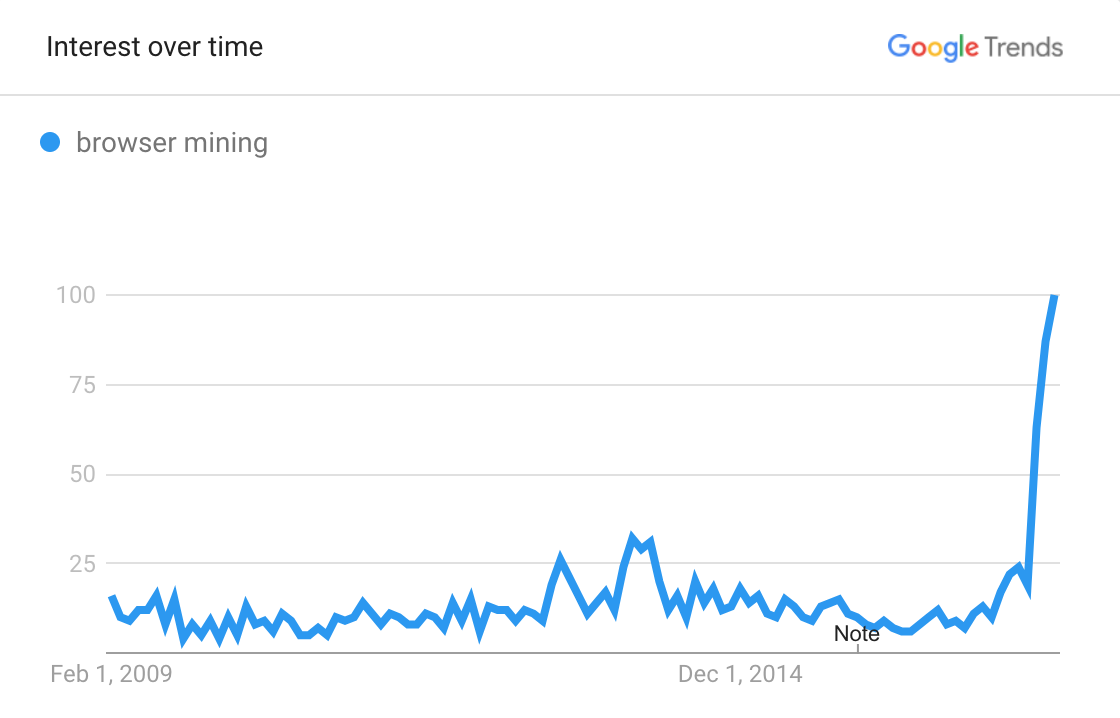
\includegraphics[width=0.75\textwidth]{browser_mining.png}}
	\caption{Search interest for ``browser mining'' over time}
\end{center}

The graph above shows how the searches for ``browser mining'' have changed since Bitcoin was launched. Search interest seems to have piqued during price surges, which culminated with Bitcoin crossing \$1000 USD for the first time in December 2013. Soon after Bitcoin`s first major crash searches consistently waned until a recent large spike, which is more than 4 times the lifetime average. The waning period before the recent surge could be attributed to the advent of ASIC usage for Bitcoin mining, and the surge is likely due to the revival of browser mining for non-Bitcoin currencies that have gained a sizeable market capitalization. As a result, websites like Showtime.com ~\cite{showtimehive}, and ThePirateBay.org ~\cite{piratesbayhive} may have experimented with browser mining as a way to add a new revenue stream.

\section{Egalitarian Proof-of-Work}

One of the mains reasons for the resurgence of this type of mining may be the recent rise in price and popularity of the cryptocurrency Monero~\cite{monero}. Launched in April 2014, Monero focuses on privacy by obfuscating the participants and amounts in transactions. This is in contrast to more popular cryptocurrencies like Bitcoin and Ethereum where transactions can be traced back through the entire blockchain. In fact, Monero gained some fame for its ability to anonymize bitcoins by converting them into Monero, transacting them privately, and then converting them back to bitcoins. This has made Monero popular on black market websites where illicit goods can be purchased without having transactions traced back to buyers. 
\\
More importantly, Monero differs in the way its currency is mined by employing a proof-of-work that is egalitarian by design. This is achieved by using the proof-of-work algorithm named CryptoNight~\cite{cryptoknight}, which makes its puzzle resistant to ASICs and fast memory-on-chip devices with low latency. While many cryptocurrencies use a similar type of proof-of-work, Monero was one of the earliest to adopt and popularize it. 
\\
Bitcoin uses SHA-256 for its hash-based proof-of-work algorithm, which is a CPU-bound function. This allows miners to use ASIC devices to increase their calculation speeds, which greatly surpasses an ordinary computer in hashes per unit of money. CryptoNight uses a memory-bound function, which relies on a situation where the time taken to complete a given computational problem is decided primarily by the amount of memory required to hold data. This limits the ability for pipelining, which is also known as instruction-level parallelism.  
\\
Satoshi Nakamoto’s original philosophy and intention for Bitcoin was “one-CPU-one-vote”~\cite{nakamoto2008bitcoin}, which CryptoNight attempts to enforce. In CryptoNight, users vote for the right order of transactions and honest money supply distribution with their CPU power, so the more CPU cores they have the more voting power they acquire. Since CPUs are relatively affordable and accessible, it follows that most users will have approximately equal voting rights. Then by relying on random access to a slow memory and emphasizing latency dependence, it is ensured that proof-of-work is largely controlled by CPUs instead of GPUs or ASICs. This is done by having every new block depended on the previous block’s solution, which must be kept in memory. This algorithm requires approximately 2MB per instance, which fits in the L3 cache per core of modern processors. Over the course of the next few years, these modern processor L3 cache sizes should become mainstream and allow more CPUs, and thus users, to vote into Monero`s ecosystem. It has also been shown that ASICs cannot handle more than 1MB of internal memory, which is less than the size of memory required to calculate a new block. GPUs are also at a disadvantage since GDDR5 memory, for example, is notably slower than L3 cache~\cite{van2013cryptonote}.  

\section{Browser Mining}
The concept of browser mining can be described as accessing CPU processing power through the JavaScript programming language on a web browser instead of a standalone native application. This allows for more scalability as there is no need to install any additional software on a computer with an internet connection. In the early days of cryptocurrency mining, there was a rise in Bitcoin JavaScript miners such as JSMiner\footnote{A JavaScript Bitcoin miner \url{https://github.com/jwhitehorn/jsMiner}}(2011) and MineCrunch\footnote{Minecrunch, web(JS) miner with integration feature\url{https://cryptocurrencytalk.com/topic/24618-minecrunch-web-js-miner-with-integration-feature/}}(2014). Minecrunch had a bigger campaign and more online presence from their developers. Based on the developer claims, the JavaScript miner was well optimized but worked 1.5x slower than CPUMiner\footnote{CPU miner for Litecoin and Bitcoin - \url{https://github.com/pooler/cpuminer}}, which was an native application to mine on CPUs. However, as the hashing power of the Bitcoin network increased the mining difficulty similarly increased, and Bitcoin CPU mining became no longer profitable. As a result, the developers stopped maintaining the codebase of such miners.
\\
As Monero became more popular, it caught the attention of some independent developers who decided to revisit the idea of browser mining. One of the earliest efforts appeared in September 2017 and was called Coinhive~\cite{coinhive}. Soon after a competitor named Crypto-Loot\footnote{Crypto-Loot - A web Browser Miner | Traffic Miner | CoinHive Alternative \url{https://crypto-loot.com/}} emerged. Both websites provided APIs\footnote{Application programming interface} to developers for implementing browser mining on their websites that used their visitors` CPU resources to mine Monero. A portion of mined Monero would go back to the API developer, and the rest would be kept by the website. Not long after their early success, several copycats appeared such as Coin-Have and PPoi~\cite{coinhivecopycats}. It even inspired a new coin specifically designed for browser mining named JSECoin\footnote{JSEcoin – Website Cryptocurrency Mining \url{https://jsecoin.com/}}. These developments took place over a few short weeks, which signalled the renewed success of browser mining. However, Coinhive`s approach as a legitimate group set it apart from its peers and established itself as the leader in the space. They also launched separate services such as proof-of-work CAPTCHAs and short-links, which could be used to prevent spam while mining Monero~\cite{coinhive}.

\section{State of affairs}
In order to find out how browser mining is changing internet use, the approach taken was to find measurements of the impact it causes. One approach was to see what the search interest over time for such services is. 

\begin{center}
	\makebox[1\textwidth]{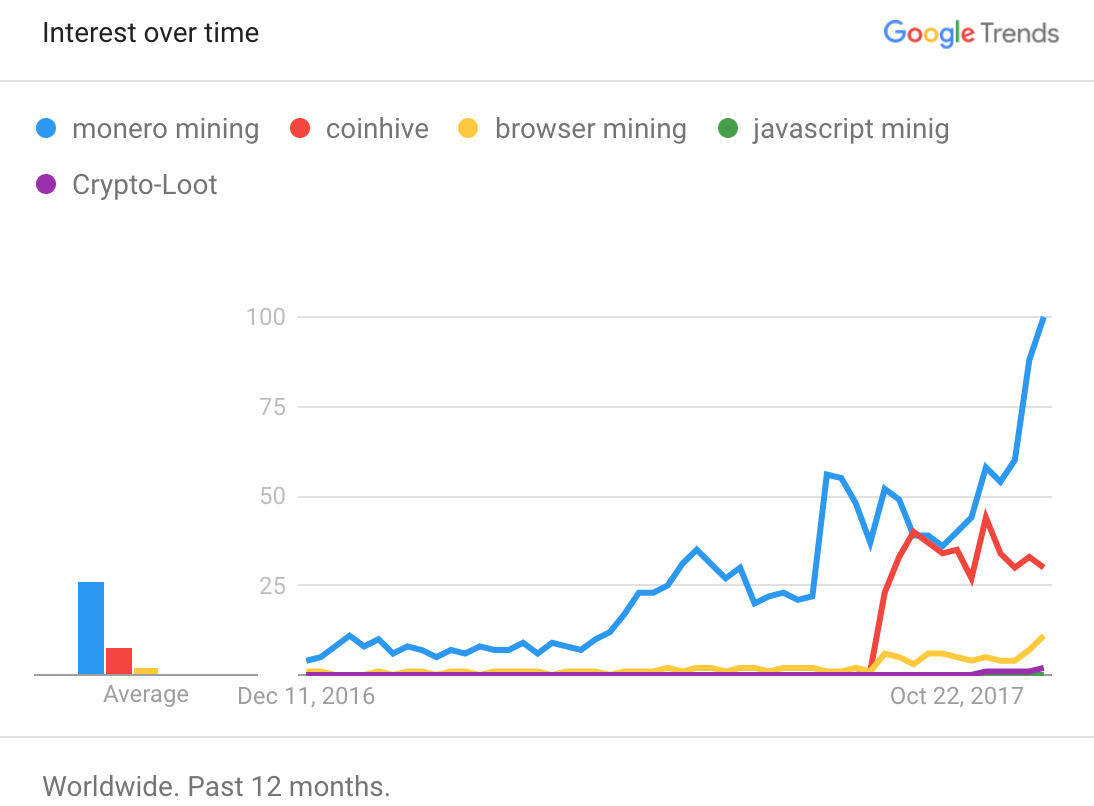
\includegraphics[width=0.75\textwidth]{usage_over_time2.png}}
	\caption{Google Trend - Search interest over last 12 months}
\end{center}

It seems that there has been more interest in Coinhive than the broader, related search term ``Browser mining''. Comparing to other services offering Monero browser mining API, Coinhive had the advantage of being the first to offer the service, hence more interest at the time of writing. There has not been enough data and evidence of usage for other services to analyze, thus the focus of this paper is on the impact of Coinhive scripts on the internet. 

The next step was to see how many websites are jumping on Coinhive's train by using Internet scanners such as Zmap\footnote{\url{https://zmap.io}}. It was of more intrest to see what the trend of this usage was, and for this purpose historical data is required. 

\begin{lstlisting}[caption={BigQuery SQL query to find websites using coinhive miner script using censys.io datasets},label={lst:bigquery},language=sql]
SELECT domain, tags, p80.http_www.get.headers.content_language, p80.http_www.get.headers.server, p80.http.get.headers.x_powered_by, p80.http.get.title , p80.http_www.get.body as wwwbody, p80.http.get.body as plainbody
FROM `censys-io.domain_public.20171123`
WHERE STRPOS(p80.http.get.body, 'coinhive.min.js') >0 or STRPOS(p80.http_www.get.body, 'coinhive.min.js') >0)
\end{lstlisting}


Using censys.io BigQuery dataset ~\cite{censys15}, it is feasible to query for such trends. The method used to gather these data is simply looking for the `coinhive.min.js` script within the body of the website page, however this could be circumvented if the website owner uses a custom version of this script (e.g. renamed hosted file).


\begin{center}
	\makebox[1\textwidth]{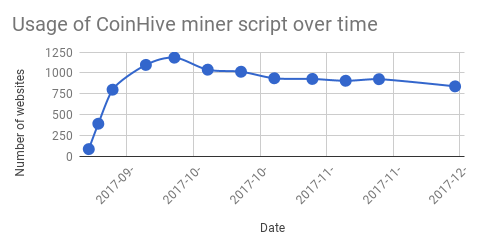
\includegraphics[width=0.75\textwidth]{usage_of_coinhive_over_time.png}}
	\caption{Usage of CoinHive Miner scripts in top 1 million websites over time}
\end{center}

As seen in the chart above, the adoptation of this script was substantial in the first days of its release. However, progress slowed down as Adblockers and organizations started to block Coinhive's website. The initial purpose of this service, as claimed by Coinhive, was to replace ads and cover server costs for webmasters. As the service did not require that website's received user consent before beginning to mine, it started to be used as maliciously in user`s browsers. This type of usage resulted in Coinhive being included in the top-10 most wanted malwares list after some famous ransomwares ~\cite{checkpoint}. 

\begin{center}
	\makebox[1\textwidth]{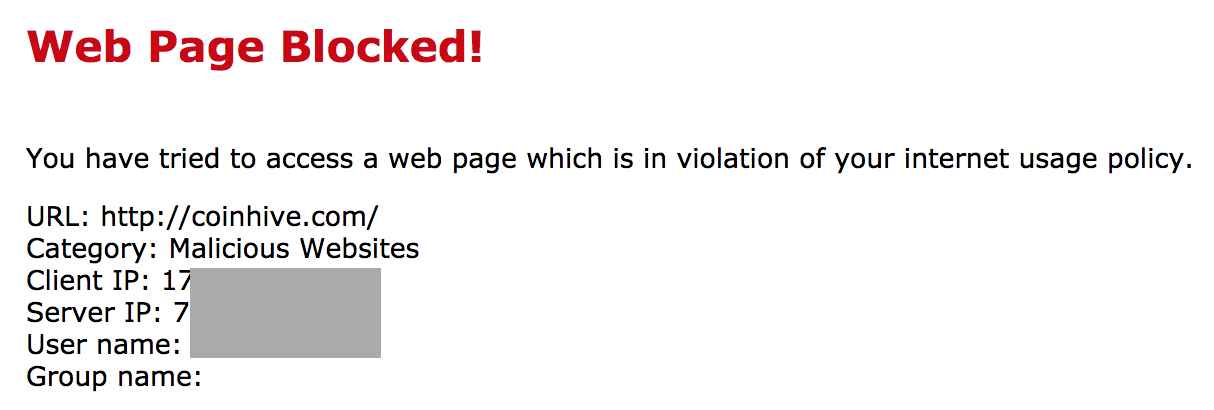
\includegraphics[width=0.5\textwidth]{coinhive_blocked.png}}
	\caption{Concordia University has blocked coinhive.com website}
\end{center}

This helped the copycats to gain some market attention, but also pushed Coinhive developers to think of other methods that would be more focused on user consent and bypassing blockage for running such scripts. Coinhive introduced another domain and service called ``Authedmine'' , which requires user`s consent to start mining in the browser. This service did not get the same attention as the original service, but it did inspire discussions regarding the ethics of such services, which is covered in Discussion section of this paper. 
%TALKED ABOUT ETHICS? UPDATE HERE

\begin{center}
	\makebox[1\textwidth]{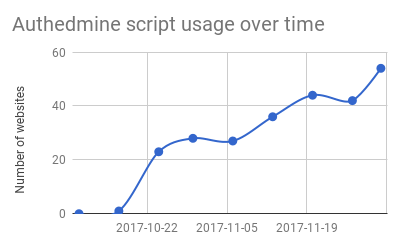
\includegraphics[width=0.75\textwidth]{usage_of_authedmine_over_time.png}}
	\caption{Usage of AuthedMine Miner scripts in top 1million websites over time}
\end{center}

Most of these scripts discovered were defaulted to use around 25\% of user`s CPU, which can be justified as it will be under the threshold of attracting the user`s attention, and it could be argued as fair-usage of their hardware. During the first few days, however, there were some reports of 100\% CPU usage when visiting websites containing these scripts~\cite{piratesbayblog}, which can be characterized as malicious.

\begin{center}
	\makebox[1\textwidth]{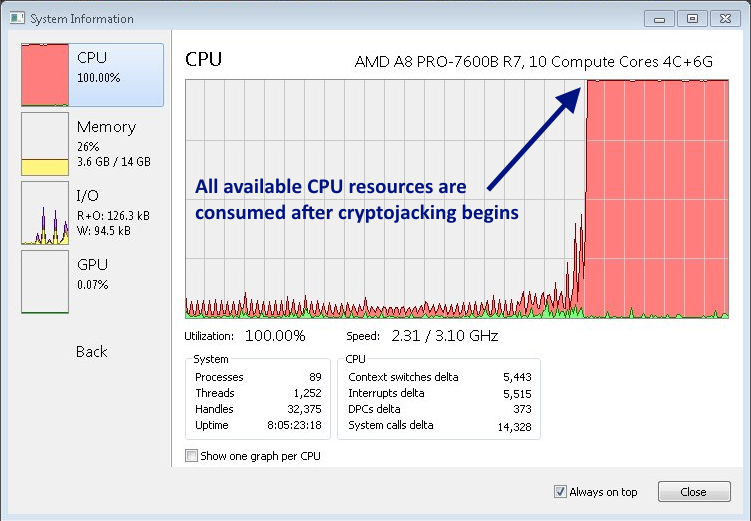
\includegraphics[width=0.75\textwidth]{windows_cpu_usage.png}}
	\caption{CPU usage browser mining scripts in the second half of the chart compared to the first half of normal use}
\end{center}

\section{Discussion}

The opinion of the authors of this paper maintain that users should be given the option to enable the miner code in their browser only with some benefit to their experience on the website.  An example of a benefit could be the removal of advertisements. Recent polls support this notion, such as the one conducted by Bleeping Computer, which found that ``many users said they are OK with websites mining Monero in the background if they don`t see ads anymore''~\cite{bleepingcomputerminers}. Another example would be granting access to premium features of the website such as journal articles behind a paywall, or streaming in high-definition. The website could also allow the user to participate in mining rewards by allocating a large portion of their CPU resources to the activity of mining, which would benefit both parties. By notifying the user of the potentials of such activity, and allowing them to make a choice to participate, the website maintains trust in their relationship with the user while also benefiting from a new source of revenue. By foregoing disclaiming this new activity, which can have harmful effects, the website will gain a new revenue stream for a short time only while sacrificing their reputation in the long term. Coinhive`s recent response to the market`s negative reaction by releasing AuthedMine, which enforces user consent before enabling any mining JavaScript code, justifies this rationale. However, before consented browser mining could develop into a sustainable model, its security implications and user impact should be addressed.

\subsection{Security}
Attack surface to abuse user`s browsers is broad. If the browsers do not block such scripts, there are different actors which can abuse this functionality for their own profit without user consent. There are multiple vectors a malicious actor can inject these scripts in the website codebase:
\begin{itemize}
\item \textbf{Website Owner:} As discussed before, the website administrator can add the script to the webpage without informing users
\item \textbf{Ad Publisher:} Similar to the claimed Showtime case~\cite{showtimehive} the advertisement publisher can inject miner script to any website they have ad space in, instead of showing ads (more on this in User Impact section).
\item \textbf{Hacked Website:} An attacker can hack the website and inject the miner code to the website codebase
\item \textbf{Man-in-the-middle attack:} Any internet service provider or free public wireless can inject the script to all the plain text traffic that goes through their routers. Ad injection has been seen in the wild ~\cite{vergeadinjection}, there has been reports of some Starbucks free wifi internet using this method of browser miner injection\footnote{\url{https://twitter.com/imnoah/status/936948776119537665}}.
\end{itemize}

\begin{center}
	\makebox[1\textwidth]{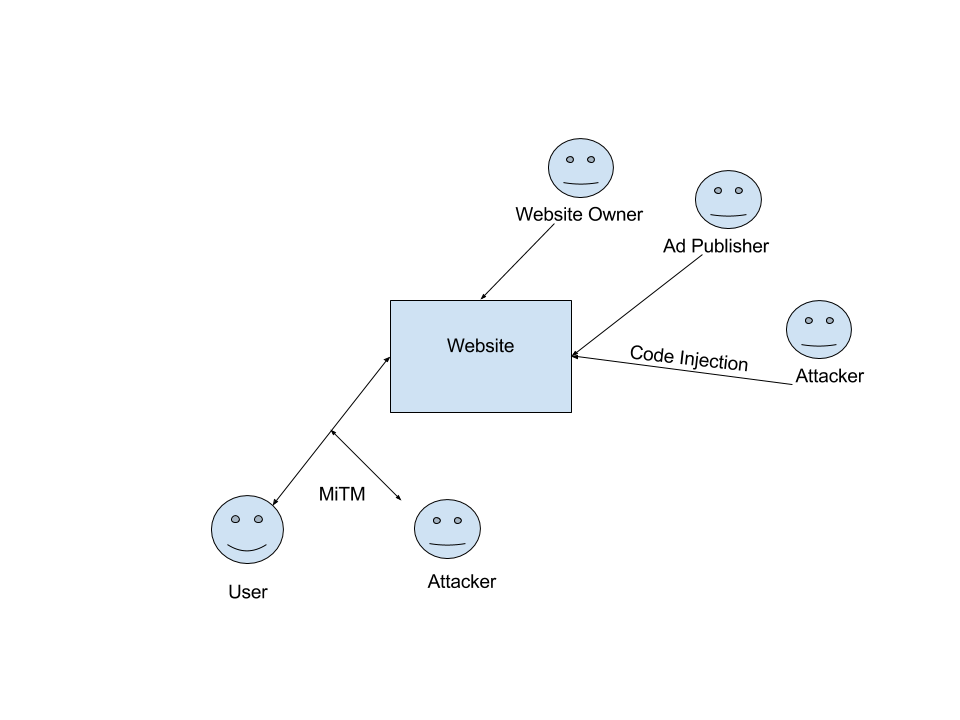
\includegraphics[width=0.5\textwidth]{attack_vectors.png}}
	\caption{Attack vectors to inject miner scripts in webpages}
\end{center}

\subsection{User Impact}

Most browser mining code is ran without the consent, nor knowledge, of the users involved. As previously mentioned, the websites that have been found running JavaScript code for the purpose of mining usually employed Coinhive`s API. One such website, for example, ThePirateBay.org~\cite{bbcmintcrypto}, which ran the JavaScript code when users searched for torrent files. Perhaps unsurprisingly, there was no notice in their Privacy Policy nor visible warning on any part of the website that informed their users of this activity. This resulted in a backlash against the website, which responded with the following statement, ``Do you want ads or do you want to give away a few of your CPU cycles every time you visit the site?'' ~\cite{piratesbayblog}. While they admitted to their testing of browser mining, their notice came after the fact and resulted in the removal of the JavaScript code altogether due to upset users. This is in contrast to the banners users are presented with upon the first visit to a website that warns them of the website`s policy on cookies, which is enforced today through EU laws~\cite{eucookie}. It is now widely known that these cookies can be used to track users across the internet, so cookie banners can act as a reminder and allow the user to make better informed decisions regarding their browsing habits. Without any type of disclaimer for users, websites have been commandeering their users` CPU resources for their business and personal gain. This results in higher energy bills for the user, along with accelerated device degradation, and slower system performance~\cite{gaurdianelectricity}.
\\
A second example of a popular website deploying Coinhive’s API is Showtime.com~\cite{gaurdianelectricity}, which is a popular cable channel that also streams their TV shows online. It was then hardly surprising when UFC.com was accused of using this very same code on the night of streaming one of their most popular events~\cite{registerufcmonero}. Both Showtime and UFC defended their actions by claiming that the miner was unknowingly activated through an ad injection. Whether this claim is true or not, the recent trend of streaming websites deploying Coinhive`s API could be due to the high costs of providing streaming services. While ads can be used to offset some of those costs, it would be of interest to some to at least experiment with the idea of recruiting their users to mine Monero for profit.
\\
Given the recent interest some websites have shown in regard to browser mining, we also see the potential for this new form of revenue generation to compete with advertisements. An immediate impact could be to reduce how many ads a user sees on a given website, and in the future it could one day even replace them. This is because the malware that is associated with advertisements is still a growing concern, and the public`s dislike of advertisements will likely persist and not wane. Also, as cryptocurrencies continue to grow in market capitalization and use cases, their inevitable mainstream use will push the profitability of mining egalitarian proof-of-work cryptocurrencies, such as Monero, well into the future. Many blogs have discussed this potential, such as the CEO of OTAMate Technology Ltd, Carl Whalley, who discussed the potential of browser mining one day replacing online advertisement~\cite{carlcryptoads}.

\section{Future Work}
%The lack of regulation in cryptocurrency space allows for a grey market to grow. This is felt more when it affects non-tech-savvy users. 

Similar to regulations for cookies and user tracking there is a need to regulate browser mining, primarly to notify users of the existence of these scripts on the webpages they visit. Also, there is a need to standardize this model, so to answer some of these questions: If every website uses a browser miner and users have many tabs open, how are CPU resources shared between them? How will the behaviour of these scripts change based on the device they are running on? If device is on power saving mode, how will that affect the execution of these scripts?

In addition to regulation and standardizing, better security design is required to narrow down the attack surface, such as using SSL/TLS and tokenizing the requests to make sure websites get user`s consent before running these scripts. 

Surveys with larger sample size and diversity is required to gauge users acceptance. These surveys should answer how much CPU power users are willing to volunteer, and if battery impact would change their affinity for participation.

Browser mining has been shown to not be as efficient as native mining applications today. Therefore, optimizations on how browsers pass system calls to the operating system can be made, or there can even be browsers designed specifically to support efficient browser mining.

This new model of monetizing websites can be a paradigm shift in how advertisement giants monopolize internet traffic. This could lead to re-democratizing the online advertisement ecosystem to make it fairer for smaller players.


%needs more here
